\documentclass{beamer}
\usefonttheme[onlymath]{serif}
\usepackage{ctex} %采用中文
\usepackage{hyperref} %超链接
%\usepackage[T0]{fontenc}

\usepackage{latexsym,xcolor,booktabs}
\usepackage{multicol}
\usepackage{graphicx,pstricks,listings,stackengine}
\usepackage{linguex,cgloss4e,tikz,qtree,tikz-qtree}
\usetikzlibrary{graphs}
\usepackage{wrapfig}
\usepackage{calligra} %英文字体中西文混排字库New Century Schoolbook
\usepackage[p,scaled=0.95]{scholax} % 0.95 适合与汉字匹配, osf 风格有效
\usepackage[scaled=.99]{helvet} % text = Helvetica = sans serif
\usepackage{amsmath,amsfonts,amssymb,amsthm} % 数学符号,要在newtxmath之前
\usepackage{mathtools}

% 设置用acrobat打开就会全屏显示
\hypersetup{pdfpagemode=FullScreen}

% 设置logo
% \pgfdeclareimage[height=0.8cm]{university-logo}{pic/logo} %需提前将logo文件放到`.tex`文件中.
% \logo{\pgfuseimage{university-logo}}

\author[Z]{Z}
\title{半导体物理期中模拟 \quad 答案}
\subtitle{Semiconductor Physics Midterm Review}
\institute[集成百川\; 同“芯”向前]{\large 集成百川\; 同“芯”向前\\njuic}
\date{\small \today}
\usepackage{NJU}

% defs
\def\cmd#1{\texttt{\color{red}\footnotesize $\backslash$#1}}
\def\env#1{\texttt{\color{blue}\footnotesize #1}}
\definecolor{deepblue}{rgb}{0,0,0.5}
\definecolor{deepred}{rgb}{0.6,0,0}
\definecolor{deepgreen}{rgb}{0,0.5,0}
\definecolor{halfgray}{gray}{0.55}

\lstset{
    basicstyle=\ttfamily\small,
    keywordstyle=\bfseries\color{deepblue},
    emphstyle=\ttfamily\color{deepred},    % Custom highlighting style
    stringstyle=\color{deepgreen},
    numbers=left,
    numberstyle=\small\color{halfgray},
    rulesepcolor=\color{red!20!green!20!blue!20},
    frame=shadowbox,
}

% defs
\def\cmd#1{\texttt{\color{red}\footnotesize $\backslash$#1}}
\def\env#1{\texttt{\color{blue}\footnotesize #1}}
\definecolor{deepblue}{rgb}{0,0,0.5}
\definecolor{deepred}{rgb}{0.6,0,0}
\definecolor{deepgreen}{rgb}{0,0.5,0}
\definecolor{halfgray}{gray}{0.55}

\usepackage{ ragged2e}
\justifying \let\raggedright \justifying

\begin{document}

%\AtBeginSection[]
%{
%\begin{frame}
% \frametitle{章节目录}
% % \begin{multicols}{2}
% %  \tableofcontents[currentsection]
% % \end{multicols}
% \tableofcontents[currentsection]
% \end{frame}
%}

%    \AtBeginSubsection[]
%    {
%     % \begin{frame}
%     % \frametitle{章节目录}
%     % \begin{multicols}{2}
%     %  \tableofcontents[currentsection]
%     % \end{multicols}
%     % \end{frame}
%    \frametitle{章节目录}
%    \begin{frame}
    %\tableofcontents[sectionstyle=show/shaded,subsectionstyle=show/shaded/hide,subsubsectionstyle=show/shaded/hide]
    %\end{frame}
    %}

\begin{frame}
    %\thispagestyle{plain}
    \maketitle
    %\titlepage

\end{frame}


\section{简答}

\begin{frame}[t]{晶体结构}
    \textbf{1. 什么是晶体点阵?和晶体结构的关系是什么?原胞取法唯一吗?}\par
    \vspace{0.2cm}
    \textbf{晶体点阵是晶体结构的抽象表示}:晶体点阵是一种数学抽象,它体现了晶体内部原子或分子的周期性排列.格点代表结构单元(基元),可以代表基元中任意一个等价的点.\par
    \textbf{晶体结构是晶体点阵的具体实现}:当晶格点阵中的格点被具体的基元(如原子、分子或离子)代替后,就形成了实际的晶体结构.因此,可以说晶体结构是晶体点阵在物理空间中的具体实现.\par
    \vspace{0.1cm}
    Lattice  + Basis  =  Crystal\par
    \vspace{0.1cm}
    原胞取法不唯一.
\end{frame}


\begin{frame}[t]{晶体结构}
    \textbf{2. 晶体的晶面是什么?密勒指数是什么(仅考虑立方晶系),该如何确定?} \par
    \vspace{0.1cm}
    \textbf{晶面}:在布拉维格子中所作的一簇互相平行的平面,平面等间距,可以将所有的格点包括无遗.\par
    \vspace{0.1cm}
    \textbf{密勒指数}:晶面指数,标定了晶面簇的方向.\par
    \vspace{0.1cm}
    \textbf{取法}:\par
    {\small  \vspace{-0.2cm}
    \begin{itemize}
    
        \item \textbf{确定截距}:在晶面簇中任选一晶面计算在三个晶胞基矢上的截距($x_1 x_2 x_3$).如果晶面与某基矢平行,则该基矢上的截距视为无穷大.

        \item \textbf{取倒数并化简}:取这些截距的倒数$1/x_i$,并将它们化为最小的简单整数比($h:k:l$).
        \item \textbf{表示晶面指数}:将这组互质的整数用圆括号括起来,即表示该晶面的密勒指数,记为($hkl$).
    \end{itemize}
    }
\end{frame}

\begin{frame}[t]{晶体结构}
    \textbf{3. 倒空间如何理解?正空间WS原胞与倒空间的第一布里渊区分别是如何选取的?}\par
    \vspace{0.1cm}
    \textbf{倒空间}:该空间倒空间若其基矢$ \{\boldsymbol{b}_1, \boldsymbol{b}_2, \boldsymbol{b}_3\} $与正空间基矢$ \{\boldsymbol{a}_1, \boldsymbol{a}_2,$ $ \boldsymbol{a}_3\} $满足
    \[
    \left.\vec{a}_i\cdot\vec{b}_j=2\pi\delta_{ij}=\left\{
    \begin{array}{cc}
        2\pi,& i=j\\
        0,& i\neq j
        \end{array}\right.\right.\quad i,j=1,2,3
    \]
    或者,对所有正格矢$\boldsymbol{R}_n$满足$ \boldsymbol{G}_{\text{h}} \cdot \boldsymbol{R}_{n}=2 \pi m \; (m\in\mathbb{Z}) $的全部$\boldsymbol{R}_{\text{h}}$的端点构成的集合.\par
    \vspace{0.1cm}
    \textbf{另一种理解}:正空间的傅里叶变换空间.
\end{frame}

\begin{frame}[t]{晶体结构}
    \textbf{3. 倒空间如何理解?正空间WS原胞与倒空间的第一布里渊区分别是如何选取的?}\par
    \vspace{0.1cm}
    从任一格点$P$出发的所有格矢的垂直平分面,最靠近格点$P$的垂直平分面所围成的包含格点$P$的最小空间.
    \begin{figure}[htbp]
        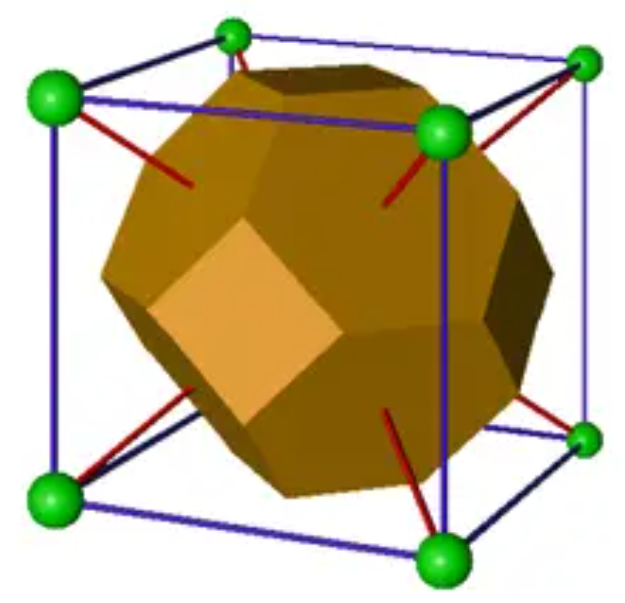
\includegraphics[width=0.3\linewidth]{1.png}
    \end{figure}
\end{frame}

\begin{frame}[t]{能带理论}
    \textbf{4. 能带理论中,周期场近似是什么?紧束缚近似是什么?布洛赫波函数是怎样的?}\par
    \vspace{-0.2cm}
    \[
    \left(-\frac{\hbar^2}{2m}\nabla^2+U(\boldsymbol{r})\right)\psi(\boldsymbol{r})=E\psi(\boldsymbol{r})
    \]
    \textbf{周期场近似}:假定单电子所感受到的势场$U(\boldsymbol{r})$具有平移对称性(周期性),即
    \[
    U(\boldsymbol{r}+\boldsymbol{R}_n)=U(\boldsymbol{r})
    \]
    \textbf{紧束缚近似}:假设原子势$V(\boldsymbol{r})$很强,晶体电子基本上是围绕着一个固定原子运动,与其他原子的相互作用很弱可以当作微扰$\Delta V$处理. \qquad 故认为$U(\boldsymbol{r}) = V(\boldsymbol{r}) + \Delta V$.\par
    \vspace{0.1cm}
    可以把紧束缚近似与近自由电子近似视作两个极端.

\end{frame}

\begin{frame}[t]{NFE vs TBA}
    \begin{figure}[htbp]
        \centering
        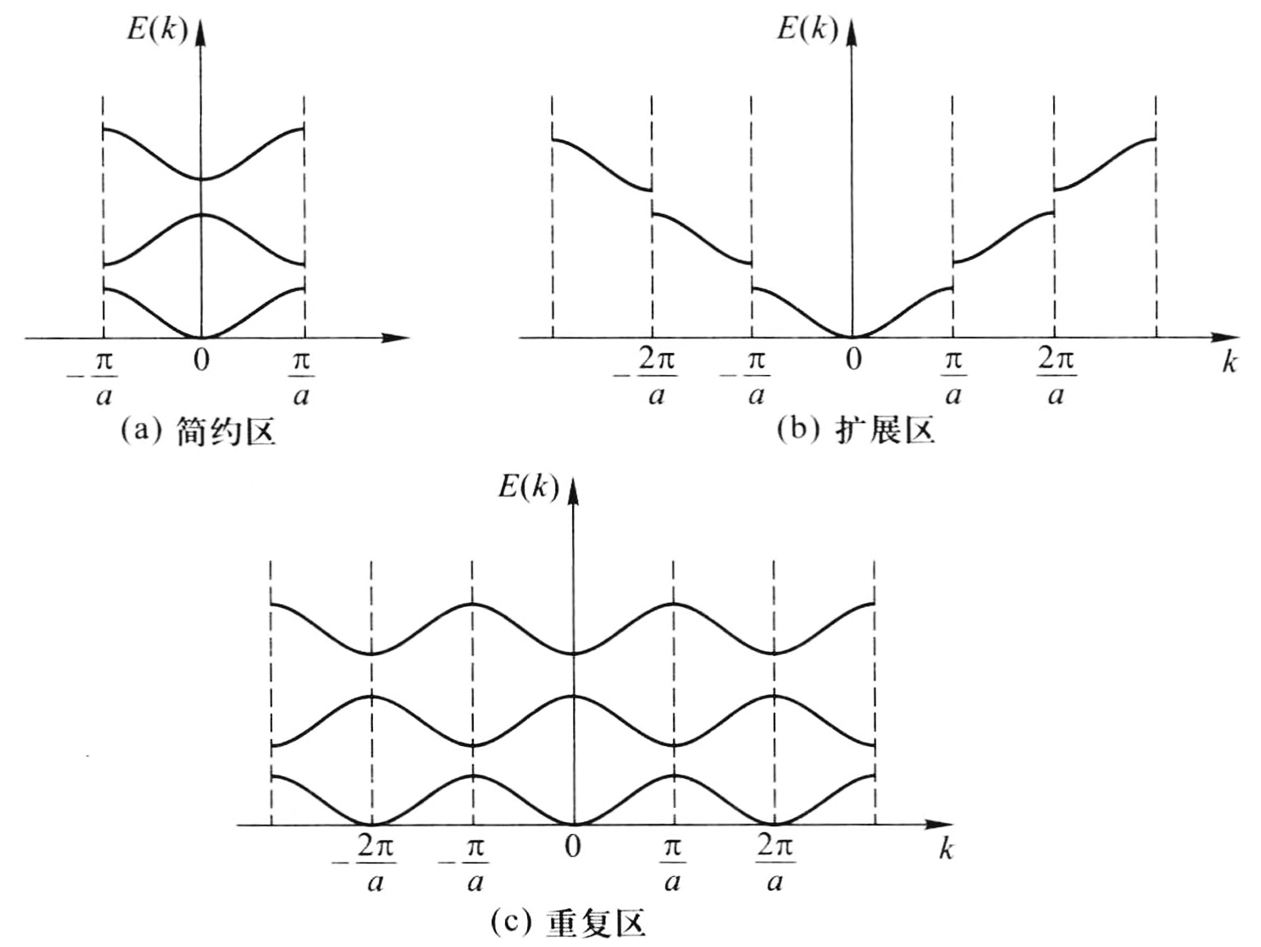
\includegraphics[width=0.75\linewidth]{2.png}
    \end{figure}
\end{frame}

\begin{frame}[t]{能带理论}
    \textbf{4. 能带理论中,周期场近似是什么?紧束缚近似是什么?布洛赫波函数是怎样的?}\par
    \vspace{-0.2cm}
    \[
    \left(-\frac{\hbar^2}{2m}\nabla^2+U(\boldsymbol{r})\right)\psi(\boldsymbol{r})=E\psi(\boldsymbol{r})
    \]
    \textbf{Bloch波函数}:若势能$U(\boldsymbol{r})$具有晶格周期性,即$U(\boldsymbol{r}+\boldsymbol{R}_n)=U(\boldsymbol{r})$,则满足上式的波函数一定具有如下形式
    \[
    \varPsi_{\boldsymbol{k}}(\boldsymbol{x})=u_{\boldsymbol{k}}(\boldsymbol{x}) \, \text{e}^{\text{i} \boldsymbol{k} \cdot \boldsymbol{x}}
    \]
    其中,$u_{\boldsymbol{k}} (\boldsymbol{x})$是与$U(\boldsymbol{r})$具有相同周期性的函数,$\boldsymbol{k}$是波矢.\par
    在周期势场中运动的单电子的波函数是调幅平面波,其振幅按晶体的周期而周期变化.
\end{frame}

\begin{frame}[t]{能带理论}
    \textbf{5. 如何理解电子共有化运动?能带是连续的吗?}\par
    \vspace{0.1cm}
    \textbf{电子共有化运动}:原子组成晶体后,不同原子的内外层波函数之间存在一定程度的交叠,故电子不再完全局限在某一个原子上,而是可以在整个晶体中运动. \par
    \vspace{0.1cm}
    能带不是连续的,是准连续的.
    \vspace{-0.1cm}
    \begin{figure}
        \centering
        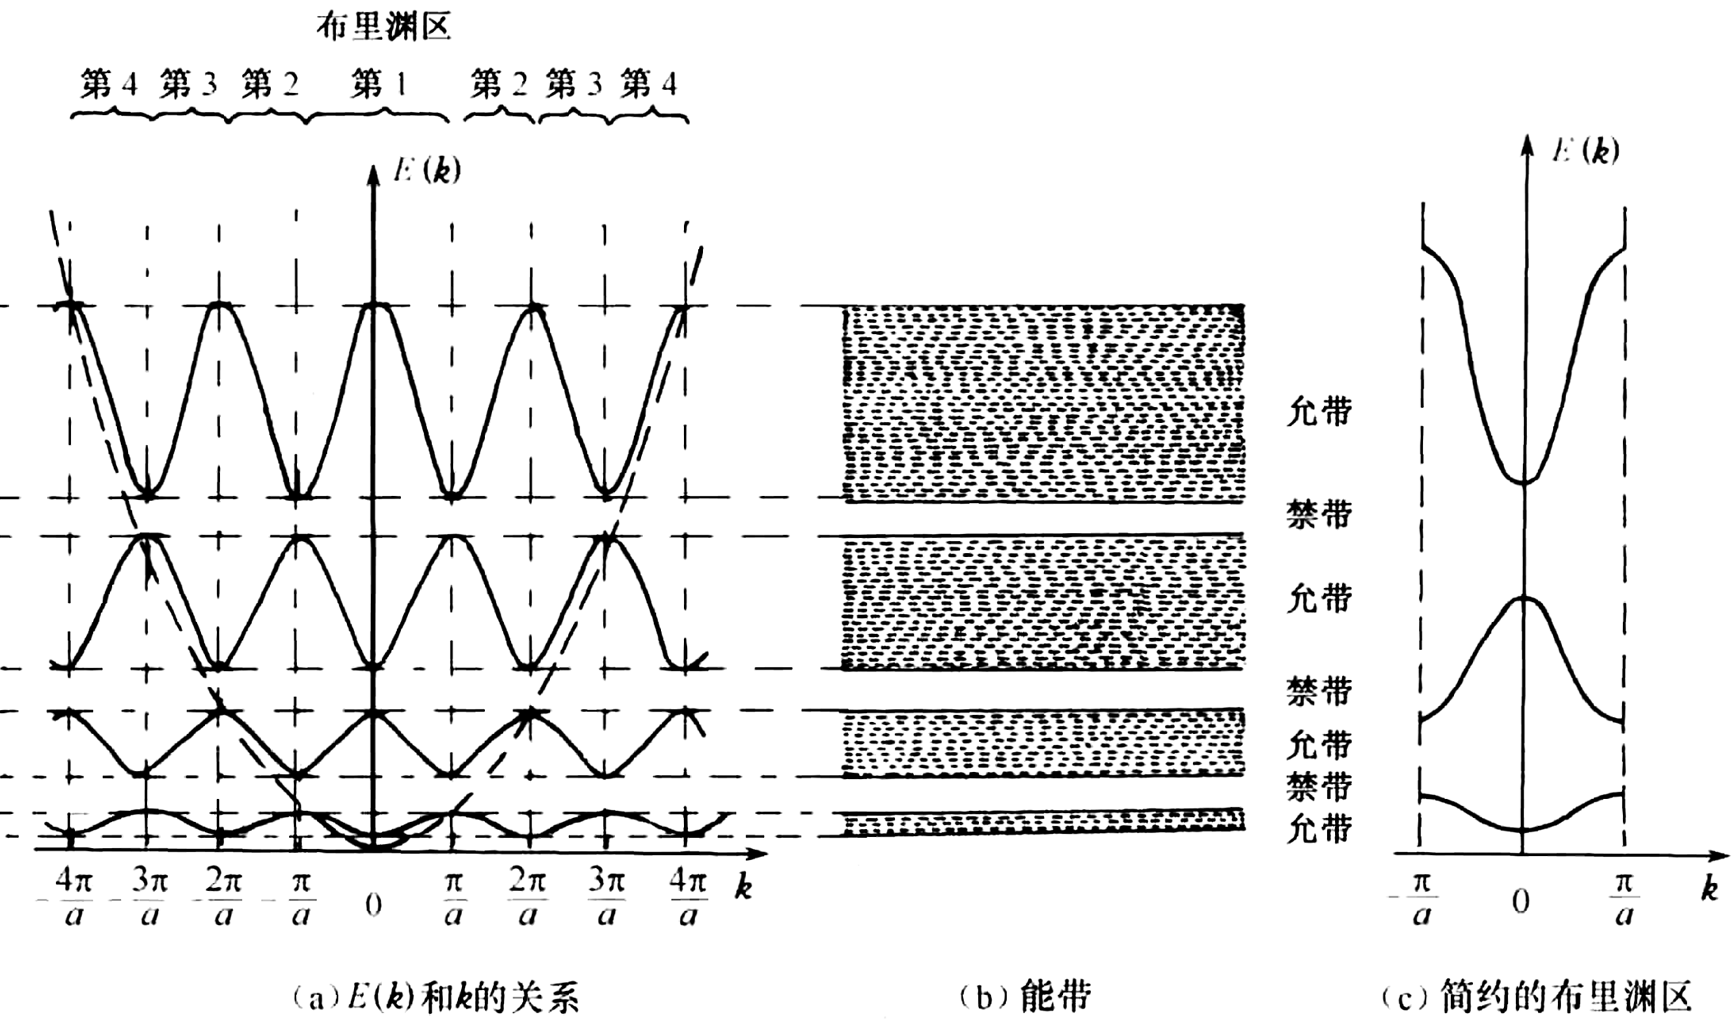
\includegraphics[width=0.6\linewidth]{3.png}
    \end{figure}
    \end{frame}

\begin{frame}[t]{能带结构}
    \textbf{6. 如何定义有效质量?其意义是什么?什么是间接带隙半导体?}\par
    \vspace{0.2cm}
    \textbf{有效质量}:在$E(k)$极值附近做泰勒展开,得到二阶项$\frac{\hbar ^2 k^2}{2m^*}$,与自由电子能量做类比得到. 可以代表能带中电子受到外力时外力与加速度关系的比例系数. \par
    \vspace{0.1cm}
    \textbf{意义}:概括了半导体内部势场对于电子的作用,使得在解决半导体中电子在外力作用下的运动规律时,可以不涉及半导体内部势场的作用. 可以引入经典力学的一些方式来分析电子.\par
    \vspace{0.1cm}
    \textbf{间接带隙半导体}:导带最小值(导带底)和价带最大值在$k$空间中处于不同位置的半导体材料.
    
\end{frame}

\begin{frame}[t]{杂质与缺陷能级}
    \textbf{7. 晶体的本征缺陷有哪些?掺杂为什么能够改变半导体导电性能?}\par
    \vspace{0.1cm}
    \textbf{本征缺陷}:点缺陷、线缺陷、面缺陷(、体缺陷).\par
    \vspace{0.1cm}
    \textbf{原因}:杂质提供了额外的载流子,同时破环了晶格周期性从而改变了能带结构,使得费米能级位置改变,从而改变了导电性.
    
\end{frame}

\begin{frame}[t]{What is Semiconductor?}
    \textbf{*. 你如何理解什么是半导体?}\par
    \vspace{0.2cm}
    \begin{itemize}
        \item 材料
        \item 电阻率
        \item 能带结构
        \item ...
    \end{itemize}
\end{frame}


\section{二}
\begin{frame}[t]{衍射分析}
    \textbf{Bragg定律} \& \textbf{Laue条件}
    \vspace{0.2cm}
    \[
    2d_{hkl}\sin \theta = n \lambda  
    \]
    \vspace{-0.3cm}
    \[
    \boldsymbol{k}_0 - \boldsymbol{k}_1 = \boldsymbol{G} 
    \]
    \vspace{-0.2cm}    
    \[
    \boldsymbol{k}_0 \cdot \boldsymbol{G} = \frac{1}{2}\boldsymbol{G}^2
    \]    
\end{frame}

\begin{frame}[t]{衍射分析}

    {
    \kaishu
    1. 常见的铝晶体是一种面心立方堆积结构,Z同学用$\lambda_1 =1.54\times  $ $10 ^{-10}$m 的X射线做衍射分析,结果得到(110)面的衍射角$\theta_1$约为$22.3^{\circ}$.请给出晶体中一个铝原子的最近邻原子数,并分析上述结果的合理性.
    } 
    
    \vspace{0.1cm}
    最近邻原子数是12.\par
    \vspace{-0.3cm}
    \[
    d_{110}=\frac{n\lambda_1}{2\sin\theta_1}=\frac{1\times1.54\times10^{-10}}{2\sin22.3^\circ}\approx2.86\times10^{-10} \text{m} \quad \text{\Large ?}
    \]
    \vspace{-0.5cm}
    \begin{figure}
        \centering
        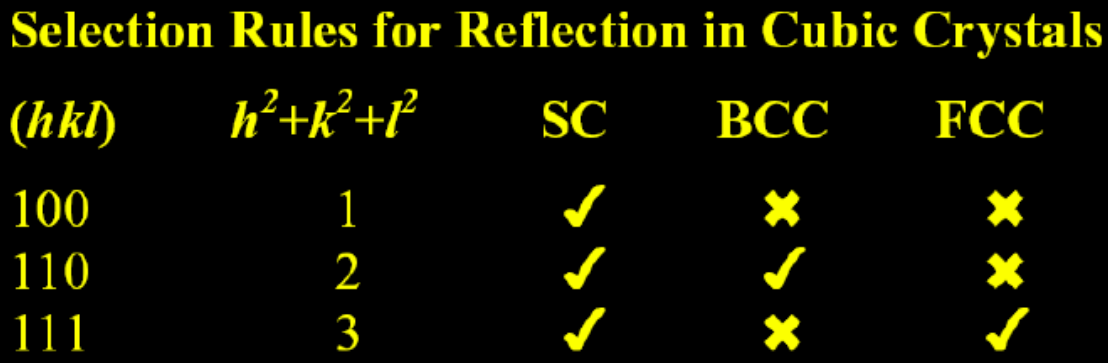
\includegraphics[width=0.7\linewidth]{4.png}

    \end{figure}
\end{frame}

\begin{frame}[t]{衍射分析}

    {
    \kaishu
    2. Z同学又使用波长$\lambda_2 = 0.071$nm 的射线对一铁晶体做衍射分析,发现随着衍射角从零开始增大,最早在$\theta_2 = 10.1^{\circ}$ 时出现衍射峰.查阅资料知常温下铁晶体结构如下,晶格常数为$2.87$\AA.请给出该衍射峰对应晶面的晶面指数,并计算铁晶体原胞的体积.
    } \par
    %\vspace{-0.2cm}
    \begin{wrapfigure}[5]{r}{2.5cm} % 纵向8行,图片靠右,宽度12.5em
    \vspace{-0.9cm}
	\begin{center}
		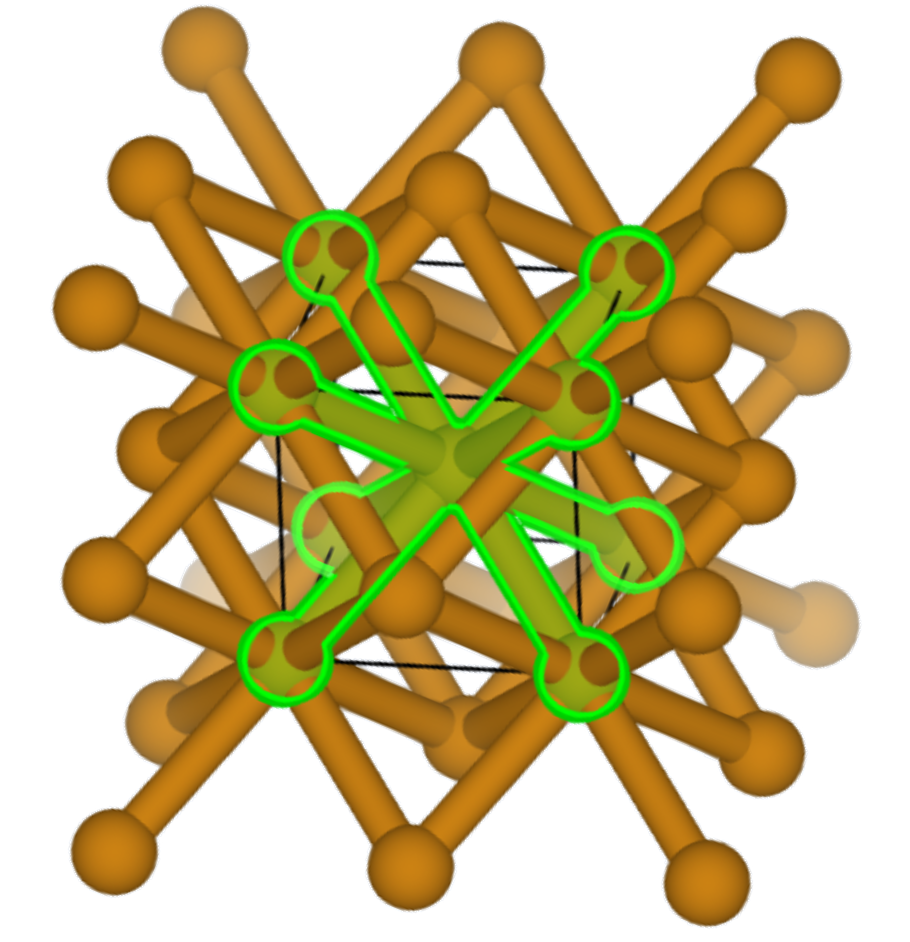
\includegraphics[width=0.93\linewidth]{5.png}
	\end{center}
    \end{wrapfigure}
    
    \vspace{0.15cm}
    \qquad 该Fe为体心立方(BCC),结合布拉格定律
    \vspace{-0.2cm}
    \begin{equation*}
        \begin{rcases}
            2\, d_{_{hkl}} \sin \theta  = n \lambda \\
            d_{_{hkl}}   = \frac{a}{\sqrt{h^2 +k^2 +l^2}}
        \end{rcases}
        \Rightarrow \sin \theta = \frac{n\lambda}{2a}\sqrt{h^2 + k^2 + l^2}
    \end{equation*}\par
    \vspace{-0.1cm}
    
    最早的衍射峰$\theta_2$对应了最小的$n\sqrt{h^2 +k^2 +l^2}$,故取$n=1$、$\sqrt{h^2 + k^2 +l^2}=\sqrt{2}$,计算有$\tilde{a}\approx 0.286$ nm $ \approx 2.87 $\AA.\par
    故晶面族为\{110\}.\par
    \vspace{0.1cm}
    原胞体积为$\frac{1}{2}a^3=1.18\times 10^{-29}$m$^3$.
    
\end{frame}

\section{三}
\begin{frame}[t]{相互作用}

    {\kaishu
    \qquad 考虑一个由两种二价离子(各$N$个,$N\rightarrow +\infty$)等间距组成的一维晶体,相互作用能为
    \vspace{-0.15cm}
    \[
    U(r)=-\frac{1}{2}\cdot 2N\Biggl[\frac{z_{1}z_{2}e^{2}}{4\pi\varepsilon_{0}r}\sum_{i(\neq j)}^{2N}(\pm\frac{1}{a_{i}})-\frac{B}{r^{n}}\Biggr]
    \]
    \vspace{-0.4cm}
    1. 请计算该晶体的Madelung常数$\alpha = \sum_{i(\neq j)}^{N}(\pm\frac{1}{a_{i}})$.\par
    }
    
    \begin{align*}
        \alpha & = \lim_{N \to \infty}2\left [ \frac{1}{1}-\frac{1}{2}+\frac{1}{3}-\frac{1}{4} + \cdots + \frac{(-1)^{N+1}}{N}\right ] \\
             & = 2\left . \sum_{n=1}^{\infty}\frac{(-1)^{n+1}}{n}x^n \right|_{x=1} \\
             & = 2 \left . \ln (1+x) \right|_{x=1}\\
             & = 2\ln 2     
    \end{align*}

\end{frame}

\begin{frame}[t]{相互作用}

    {\kaishu
    \qquad 考虑一个由两种二价离子(各$N$个,$N\rightarrow +\infty$)等间距组成的一维晶体,相互作用能为\par
    
    \vspace{-0.3cm}
    
    \[
        U(r)=-\frac{1}{2}\cdot 2N\Biggl[\frac{z_{1}z_{2}e^{2}}{4\pi\varepsilon_{0}r} 2\ln 2 - \frac{B}{r^{n}}\Biggr]
    \]
    \par
    
    \vspace{-0.1cm}
    
    2. 若$n=4$,请计算单离子的结合能$E=u(r_0)$,可用平衡间距$r_0$表示.\par
    }
    \vspace{0.1cm}
    \qquad 计算$\left.\dfrac{\text{d} U}{\text{d} r}\right|_{r_{0}}=0$,有$B = \dfrac{z_{1} z_{2} \alpha e^{2}}{4 \pi \varepsilon_{0} n} r_{0}^{n-1} = \dfrac{e^{2}r_0^3 \ln 2}{2 \pi \varepsilon_{0} }$

    \[
        \Rightarrow \quad U(r_0)= - N \frac{3e^{2} \ln 2}{2 \pi \varepsilon_{0} r_0}
    \]
    或者利用结论$U(r_0)=-\dfrac{1}{2} \cdot 2N \dfrac{z_{1} z_{2} \alpha e^{2}}{4 \pi \varepsilon_{0} r_{0}}\left(1-\dfrac{1}{n}\right)= - N \dfrac{3e^{2} \ln 2}{2 \pi \varepsilon_{0} r_0}$.
    
\end{frame}

\begin{frame}[t]{相互作用}

    {\kaishu
    \qquad 考虑一个由两种二价离子(各$N$个,$N\rightarrow +\infty$)等间距组成的一维晶体,相互作用能为\par
    
    \vspace{-0.3cm}
    
    \[
        U(r)=-\frac{1}{2}\cdot 2N\Biggl[\frac{z_{1}z_{2}e^{2}}{4\pi\varepsilon_{0}r} 2\ln 2 - \frac{B}{r^{n}}\Biggr]
    \]
    \par
    
    \vspace{-0.1cm}
    
    2. 若$n=4$,请计算单离子的结合能$E=u(r_0)$,可用平衡间距$r_0$表示.\par
    }
    \vspace{0.1cm}
    \qquad 单粒子结合能需要除以粒子数量$2N$.\par
    \vspace{-0.5cm}
    \begin{align*}
        U(r_0) & = - N \frac{3e^{2} \ln 2}{2 \pi \varepsilon_{0} r_0} \\
        \Rightarrow \quad E & = u(r_0)= \frac{U(r_0)}{2N} = - \frac{3e^{2} \ln 2}{4 \pi \varepsilon_{0} r_0}    
    \end{align*}
    \par
    \vspace{-0.3cm}
    \qquad (或许需要考虑符号的问题)
\end{frame}

\begin{frame}[t]{相互作用}

    {\kaishu
    3. 若$r_0=0.3$nm,结合能$E=3$ eV,试求$B$.\par
    }
    \vspace{-0.1cm}

    \begin{equation*}
        \begin{rcases}
            B = \dfrac{e^{2}r_0^3 \ln 2}{2 \pi \varepsilon_{0} } \\
            E = \dfrac{3e^{2} \ln 2}{4 \pi \varepsilon_{0} r_0}
        \end{rcases}
        \Rightarrow B = \dfrac{2r_0^4}{3}E
    \end{equation*}
    计算有$B=2.60\times 10^{-58}\text{J}\cdot\text{m}^4$或$1.62\times 10^{-2} \text{eV}\cdot \text{nm}^4$
    
\end{frame}

\section{四}
\begin{frame}[t]{半导体掺杂}

    {\kaishu
        \qquad 考虑室温300 K环境下一硅材料,其$N_{\text{c}}=2.8\times 10^{19}$cm$^{-3}$,$E_\text{{g}} = 1.12$eV.\par
        1. 半导体中首先掺杂了磷原子,使其费米能级来到导带底部下侧0.3 eV处,试计算磷的掺杂浓度并绘制能带图,体现出电离过程. 设杂质磷的电离能为0.04 eV.\par
    }
    \vspace{0.1cm}
    \qquad 由题意,$E_{\text{c}}-E_{\text{F}}=0.3$ eV. 结合$\Delta E_\text{D}=0.04$ eV,有\par
    \vspace{-0.3cm}
    \[
        E_{\text{D}}-E_{\text{F}}=0.26\text{eV} \gg k_0 T
    \]
    故材料在强电离区,$n_0 \approx n_{\text{D}}^+ \approx N_{\text{D}}$.\par
    \vspace{-0.1cm}
    \[
        N_{\text{D}}\approx n_0 = N_{\text{c}} \exp ( - \frac{E_{\text{c}}-E_{\text{F}}}{k_0 T} ) \approx 2.6\times 10^{14} \, \text{cm}^{-3}  
    \]
\end{frame}

\begin{frame}[t]{半导体掺杂}

    {\kaishu
        \qquad 考虑室温300 K环境下一硅材料,其$N_{\text{c}}=2.8\times 10^{19}$cm$^{-3}$,$E_\text{{g}} = 1.12$eV.\par
        1. 半导体中首先掺杂了磷原子,使其费米能级来到导带底部下侧0.3 eV处,试计算磷的掺杂浓度并绘制能带图,体现出电离过程. 设杂质磷的电离能为0.04 eV.\par
    }
    \vspace{-0.3cm}
    \begin{figure}
        \centering
        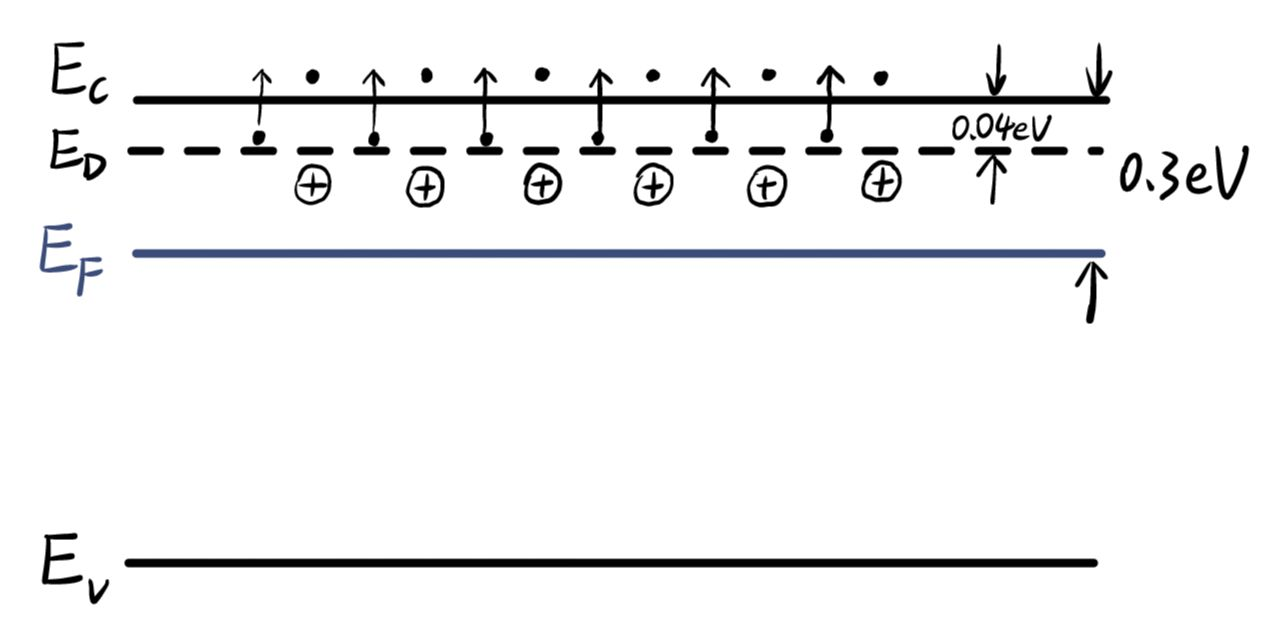
\includegraphics[width=0.75\linewidth]{6.jpg}
    \end{figure}
\end{frame}

\begin{frame}[t]{半导体掺杂}

    {\kaishu
        \qquad 考虑室温300 K环境下一硅材料,其$N_{\text{c}}=2.8\times 10^{19}$cm$^{-3}$,$E_\text{{g}} = 1.12$eV.\par
        2. 对上述硅继续掺杂硼原子,使得费米能级降低了0.1 eV,试计算硼的掺杂浓度. 假设均能全部电离.\par
    }
    \vspace{0.1cm}
    \qquad 由题意,$E_{\text{c}}-E_{\text{F}}'=0.4$ eV. 由于全部电离,视$n_0 = N_{\text{D}} - N_{\text{A}} $.\par
    \vspace{-0.2cm}
    \[
        N_{\text{D}} - N_{\text{A}} = N_{\text{c}} \exp ( - \frac{E_{\text{c}}-E_{\text{F}}'}{k_0 T} ) \approx 5.3\times 10^{12} \, \text{cm}^{-3}  
    \]
\end{frame}

\begin{frame}[t]{半导体掺杂}

    {\kaishu
        3. 请简述下列各个能带图分别表明半导体处于何种掺杂情况,并分别指出哪个符合上述1、2小题的半导体掺杂情况.\par
    }
    \vspace{-0.2cm}
    \begin{figure}
        \centering
        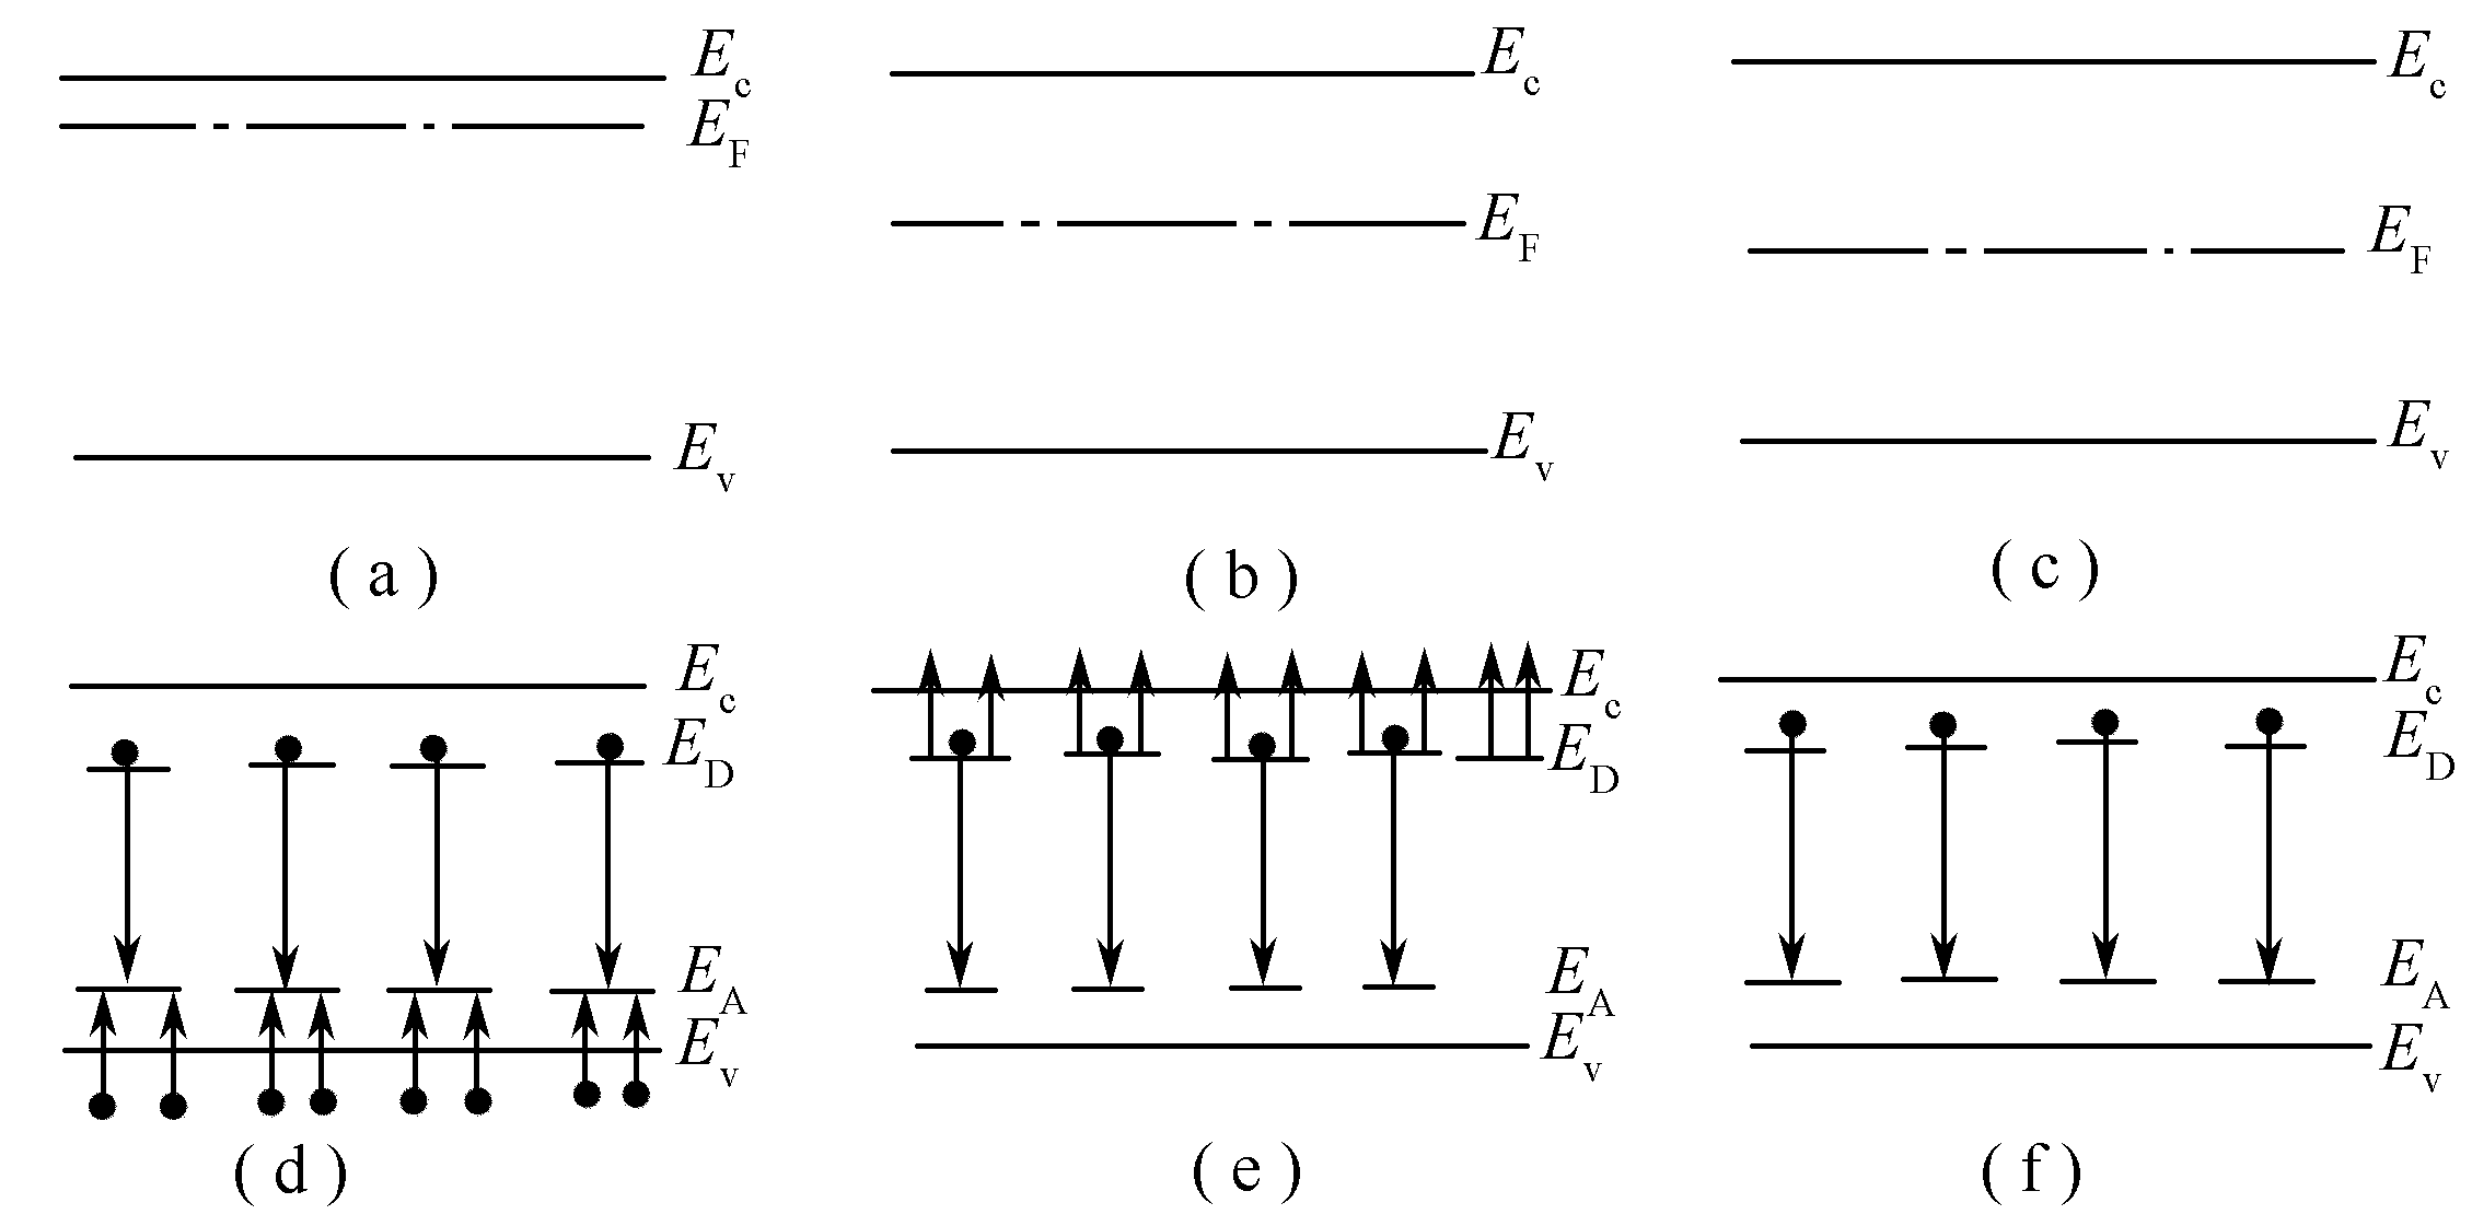
\includegraphics[width=0.7\linewidth]{7.png}
    \end{figure}
    (a) 强n型掺杂;(b) 弱n型掺杂;(c) 本征半导体\par
    (d) 受主多于施主;(e) 施主多于受主;(f) 施主与受主恰好相等.
    
    
\end{frame}

\section{五}

\begin{frame}[t]{杂质电离}

    {\kaishu
        \qquad 一杂质补偿硅材料,已知掺入受主密度$N_\text{A} =1\times10^{15} \text{cm}^{-3}$,室温下测得其$E_\text{F}$恰好与$E_\text{D}$重合,并得知平衡电子密度为$n_0$ $=$ $5\times10^{15}\text{cm}^{-3}$.已知室温下硅的本征载流子密度$1\times10^{10}\text{cm}^{-3}$,导带底有效态密度$2.8\times10^{19}\text{cm}^{-3}$.\par
        \vspace{0.1cm}
        1. 请计算平衡少子浓度与$E_\text{F}$的位置.\par
    }
    \vspace{-0.1cm}

    \[
        p=\frac{n_{\text{i}}^2}{n_0} = 2 \times 10^4 \, \text{cm}^{-3}
    \]
    由$n_0=N_{\text{c}}\exp (-\dfrac{E_{\text{c}} - E_{\text{F}}}{k_0 T})$,可计算\par
    \vspace{-0.1cm}
    \[
        E_{\text{F}} = E_{\text{c}} + k_0 T \ln \frac{N_{\text{c}}}{n_0} = E_{\text{c}} - 0.22 \, \text{eV} 
    \]
    \par
    \vspace{-0.1cm}
    同时知,$E_{\text{F}}\gg E_{\text{A}}$,故受主强电离.
    
    
\end{frame}

\begin{frame}[t]{杂质电离}

    {\kaishu
        \qquad 一杂质补偿硅材料,已知掺入受主密度$N_\text{A} =1\times10^{15} \text{cm}^{-3}$,室温下测得其$E_\text{F}$恰好与$E_\text{D}$重合,并得知平衡电子密度为$n_0$ $=$ $5\times10^{15}\text{cm}^{-3}$.已知室温下硅的本征载流子密度$1\times10^{10}\text{cm}^{-3}$,导带底有效态密度$2.8\times10^{19}\text{cm}^{-3}$.\par
        \vspace{0.1cm}
        2. 请计算掺入材料中的施主杂质浓度以及电离程度.\par
    }
    \vspace{0.1cm}
    \qquad 由$E_{\text{F}}=E_{\text{D}}$,可知$1-f_{\text{D}}(E)=\frac{1}{1+2\exp  (\frac{E_{\text{F}}-E_{\text{D}}}{k_0 T} )} = \dfrac{1}{3}$为电离程度,结合电荷平衡有\par
    \vspace{-0.2cm}
    \[
        n_0+N_{\text{A}}=n_{\text{D}}^+ = N_{\text{D}}[1-f_{\text{D}}(E)] = \dfrac{N_{\text{D}}}{3}
    \]
    而$n_{\text{D}}^+ = N_{\text{D}} - n_{\text{D}}$,可计算\par
    \vspace{-0.2cm}
    \[
        N_\text{D}=3( n_0+N_\text{A} )=1.8\times10^{16} \, \text{cm}^{-3}
    \]
\end{frame}

\begin{frame}[t]{杂质电离}

    {\kaishu
        \qquad 一杂质补偿硅材料,已知掺入受主密度$N_\text{A} =1\times10^{15} \text{cm}^{-3}$,室温下测得其$E_\text{F}$恰好与$E_\text{D}$重合,并得知平衡电子密度为$n_0$ $=$ $5\times10^{15}\text{cm}^{-3}$.已知室温下硅的本征载流子密度$1\times10^{10}\text{cm}^{-3}$,导带底有效态密度$2.8\times10^{19}\text{cm}^{-3}$.\par
        \vspace{0.1cm}
        3. 已知$N_\text{c}\propto T^{\frac{3}{2}}$,证明强电离时有{\color{red}{$E_\text{F}= $ $ E_\text{c}+kT \ln \dfrac{N_\text{D}-N_\text{A}}{N_\text{c}}$}},并简单说明该硅材料在$T=400$K 时的电离情况.\par
    }
    \vspace{0.1cm}
    \qquad 强电离区,$n_0 = N_\text{D} - N_\text{A}$,结合下式易证明.\par
    \vspace{-0.2cm}
    \[
        n_0 = N_\text{c} \exp (\dfrac{E_\text{F}-E_\text{c}}{k_0 T})
    \]
    \qquad 升温至400K,若$E_\text{F}$不变,由上式\par
    \vspace{-0.2cm}
    \[
        n_0' = 6.66\times 10 ^{16} \, \text{cm}^{-3} > N_\text{D} - N_\text{A}
    \]
    
\end{frame}

\begin{frame}[t]{杂质电离}

    {\kaishu
        3. 已知$N_\text{c}\propto T^{\frac{3}{2}}$,证明强电离时有{\color{red}{$E_\text{F}= $ $ E_\text{c}+kT \ln \dfrac{N_\text{D}-N_\text{A}}{N_\text{c}}$}},并简单说明该硅材料在$T=400$K 时的电离情况.\par
    }
    \vspace{0.1cm}
    \qquad 若升温至400K,杂质均强电离\par
    \vspace{-0.2cm}
    \[
        E_\text{F}= E_\text{c} + k_0 T \ln \dfrac{N_\text{D}-N_\text{A}}{N_\text{c}} = E_\text{c} - 0.27 \text{eV}
    \]
    下式检验$f_\text{D}(E)$,不满足强电离,实际$E_\text{F}$要降低.\par
    \vspace{-0.2cm}
    \[
        f_\text{D}(E) = \cfrac{1}{1+\cfrac{1}{2}\exp(\cfrac{E_\text{D}-E_\text{F}}{k_0 T})} = 0.33 > 0.1
    \]
    \qquad 再检验本征载流子浓度变化后得出,施主仍然中等电离,但电离程度近翻倍;受主仍然强电离.
    
\end{frame}

\begin{frame}[t]{杂质电离}
    \qquad 弱电离至强电离区,有\par
    \vspace{-0.2cm}
    \[
        N_\text{A} + N_\text{c}\exp (-\dfrac{E_\text{c}-E_\text{F}}{k_0 T}) = \dfrac{N_\text{D}}{1 + 2\exp (-\dfrac{E_\text{D}-E_\text{F}}{k_0 T})}
    \]
    \par
    \vspace{-0.15cm}
    
    \qquad 令$x = \dfrac{N_\text{c}}{2 N_\text{D}} \exp (-\dfrac{E_\text{c}-E_\text{D}}{k_0 T})$、$y = 2 \exp (-\dfrac{E_\text{D}-E_\text{F}}{k_0 T})$. 400K 下,$x = 1.850$. 则上式变为\par
    
    \[
        \dfrac{1}{18} + xy = \dfrac{1}{1+y}
    \]
    \par
    
    \vspace{-0.15cm}
    
    解得$y = 0.3658 $,进一步计算有 $E_\text{F} - E_\text{D} = -0.0586$ eV 、$n_0'=1.22 \times 10^{16}\, \text{cm}^{-3}$.
    
\end{frame}

\section{六}
\begin{frame}[t]{电离分析}

    {
    \kaishu
    \qquad Z同学采购了两块硅材料,是杂质相同但浓度不同的两块n型硅.测量得到其电子浓度与温度的关系如图所示.\par
    1. 两样品掺杂浓度较高的是哪个,在$T_A$左侧为什么两曲线近似重合.
    } \par
    
    \vspace{0.1cm}
    %\vspace{-0.2cm}
    \begin{wrapfigure}[6]{r}{5cm} % 纵向8行,图片靠右,宽度12.5em
    \vspace{-0.7cm}
	\begin{center}
		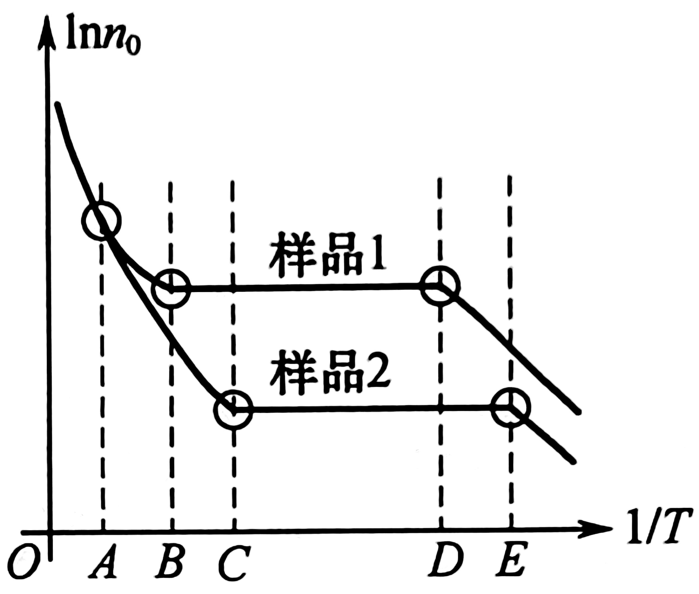
\includegraphics[width=0.93\linewidth]{8.png}
	\end{center}
    \end{wrapfigure}
    
    \qquad 样品1掺杂浓度更高. \par
    
    \qquad 在 $ T_\text{A} $ 以左区域,两 样品 处在高温本征激发区,本征激发产生的载流子数远多于杂质电离产生的载流子数,掺杂浓度对载流子浓度几乎无影响,故两曲线近似重合.
    
\end{frame}

\begin{frame}[t]{电离分析}

    {
    \kaishu
    \qquad Z同学采购了两块硅材料,是杂质相同但浓度不同的两块n型硅.测量得到其电子浓度与温度的关系如图所示.\par
    2. 两曲线在$T_C$与$T_D$之间为什么近乎平行,为什么两平行曲线的起点$T_B$、$T_C$的不一致,终点$T_D$、$T_E$也不一致.
    } \par
    
    \vspace{0.1cm}
    %\vspace{-0.2cm}
    \begin{wrapfigure}[9]{r}{5cm} % 纵向8行,图片靠右,宽度12.5em
    \vspace{-0.7cm}
	\begin{center}
		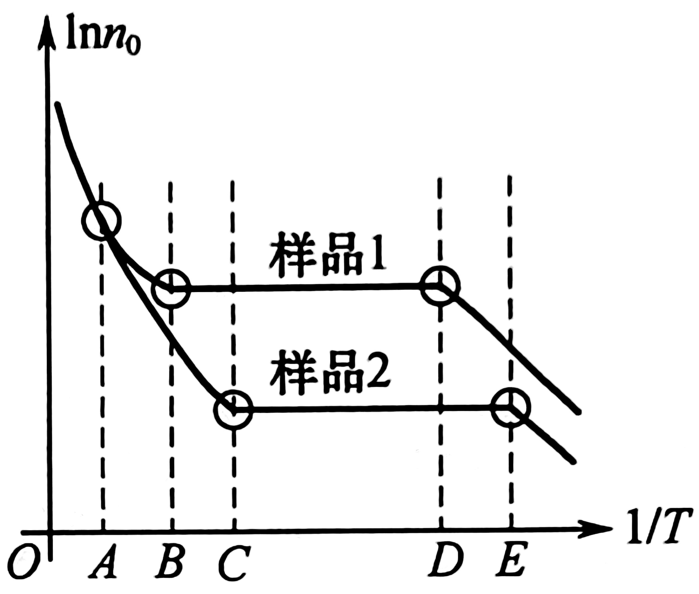
\includegraphics[width=0.93\linewidth]{8.png}
	\end{center}
    \end{wrapfigure}
    
    
    \qquad $T_C$与$T_D$之间两种样品均处于强电离区域,杂质几乎全部电离,且远大于本征激发程度,因此载流子数量基本不发生变化,故两条曲线趋于平行.\par
    
    \qquad 样品杂质浓度越高,本征激发起主要作用的温度也越高,因此$T_B$在$T_C$左侧;达到强电离的温度也越高,因此$T_D$在$T_E$左侧.
    
\end{frame}

\begin{frame}[t]{电离分析}

    {
    \kaishu
    \qquad Z同学采购了两块硅材料,是杂质相同但浓度不同的两块n型硅.测量得到其电子浓度与温度的关系如图所示.\par
    3. 若低温下,$N_{\text{c}}$近乎不变,则在$T_E$右侧两曲线是否平行,其斜率的含义是什么.
    } \par
    
    \vspace{0.1cm}    
    
    \qquad 低温电离区,有\par
    \vspace{-0.5cm}

    \begin{align*}
        \begin{rcases}
            E_{\text{F}} =\cfrac{E_{\text{c}}+E_{\text{D}}}{2}+\cfrac{k_{0} T}{2} \ln \cfrac{N_{\text{D}}}{2 N_{\text{c}}}  \\
             n_0 = N_\text{c} \exp (-\dfrac{E_{\text{c}}-E_{\text{F}}}{k_0 T})
        \end{rcases}
        \Rightarrow \; \ln n_0 =\frac{1}{2} \ln \frac{N_\text{D}N_\text{c}}{2} - \frac{\Delta E_\text{D}}{2 k_0 T}
    \end{align*}

    \vspace{-0.1cm}
    
    由于低温下$N_\text{c}$保持不变,故有直线$\ln n_0 — 1/T$,斜率为$- \cfrac{\Delta E_\text{D}}{2 k_0}$.
    
\end{frame}

\begin{frame}[t]{电离分析}

    {
    \kaishu
    \qquad Z同学采购了两块硅材料,是杂质相同但浓度不同的两块n型硅.测量得到其电子浓度与温度的关系如图所示.\par
    4. 请直接在图中绘制样品2的本征载流子浓度与温度的关系(纵坐标为$\ln n_{\text{i}}$).
    } \par
    
    \begin{figure}[htbp]
        \centering
        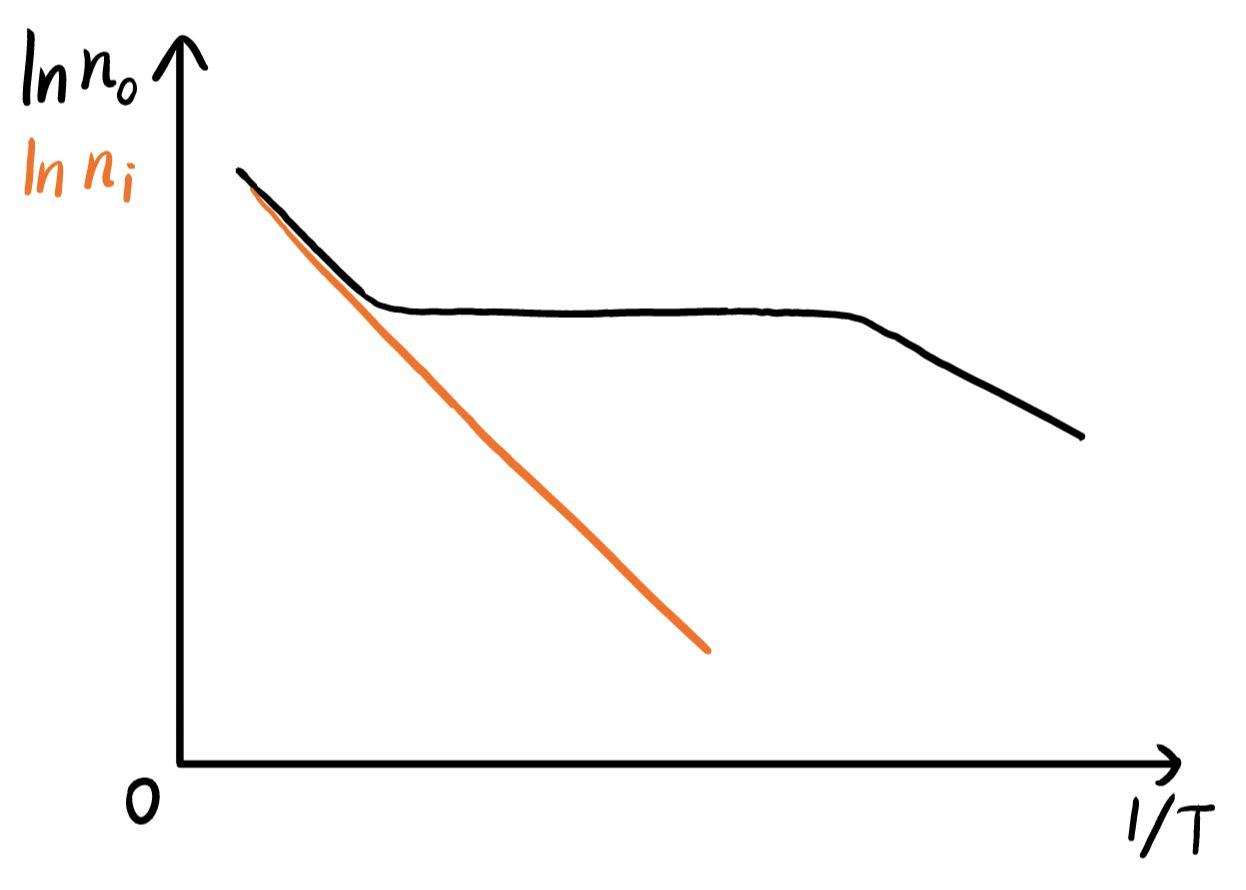
\includegraphics[width=0.6\linewidth]{9.jpg}

    \end{figure}    
    
\end{frame}

\section{七}
\begin{frame}[t]{导电率}

    {
        \kaishu
        \qquad Z同学有一个n型锗样品,在300K环境下,其电子浓度$n_0=5\times10^{14}\text{cm}^{-3}$,试计算上述温度时掺杂锗的电导率$\sigma$.已知$\mu_\text{n}=3800 \text{cm}^2/(\text{V}·\text{s})$、$ \mu_\text{p}=1900 \text{cm}^2/(\text{V}·\text{s})$、$ n_\text{i}=2.33×10^{12}\text{cm}^{-3}$.
    }\par

    \vspace{0.2cm}
    \qquad 少子浓度\par
    \vspace{-0.1cm}
    \[
        p_0 = \frac{n_\text{i}^2}{n_0} = 1.086 \times 10^{10} \text{cm}^{-3}
    \]
    \vspace{-0.1cm}
    故\par
    \[
        \sigma = n_0 q \mu_\text{n} + p_0 q \mu_\text{p} = 0.304 \, \text{S/cm}
    \]
    
\end{frame}

\begin{frame}
    \thispagestyle{empty}
    \begin{center}
        \vspace{1.75cm}
        {\Huge\calligra Thanks!}\par
        \vspace{1.5cm}
        {\Large \calligra Z}
    \end{center}
\end{frame}

\end{document}